
\section{Cartpole Outcomes}
The first task developed was the classic cartpole environment,
this was helpfull in understanding core concepts of reinforcement learning and neural networks, along with it,
cartpole was essential in testing and setting up the logging interface as well as testing different implementations of the learning algorithm 
\subsection*{Keras-rl}
Keras-rl is a community maintained high level implementation of keras agents for reinforcement learning. 
this was the first implementaiton tested.
%%%%%%%%% INSERT DETAILS HERE %%%%%%%%%

The implementation of keras-rl is very easy and doesn't require a deep understanding of reinforcement learning and the leanring structures.
\subsection*{Keras API}
The second implementaiton tested was using the plain keras API, while this provides more flexibility it also requires a much deeper understandng of how reinforcement learning works.
%%%%%%%%% INSERT DETAILS HERE %%%%%%%%%
The implementaiton using the Keras API was essential to develop a necessary knowledge for the project and to progress to the next stage.
\subsection*{}

While an implementaiton using Keras-rl would be simpler and even possibly ease the itteration process, this implementation provides less flexibility and given the target of the project and 
desire to develop a deeper understanding of reinforcement learning the implementation using the Keras API was choosen to implemnt the next phases.

\subsection*{Results}
The cartpole served as an innitial testing environment for multiple variables and strategies.

The first attempt uses Boltzmann distribution as an exploration policy %try to explain what Boltzmann is%
in this experiment an itteration on the learning rate was performed, along with the number of steps to achieve the target.

\begin{figure}[H]
    \centering
    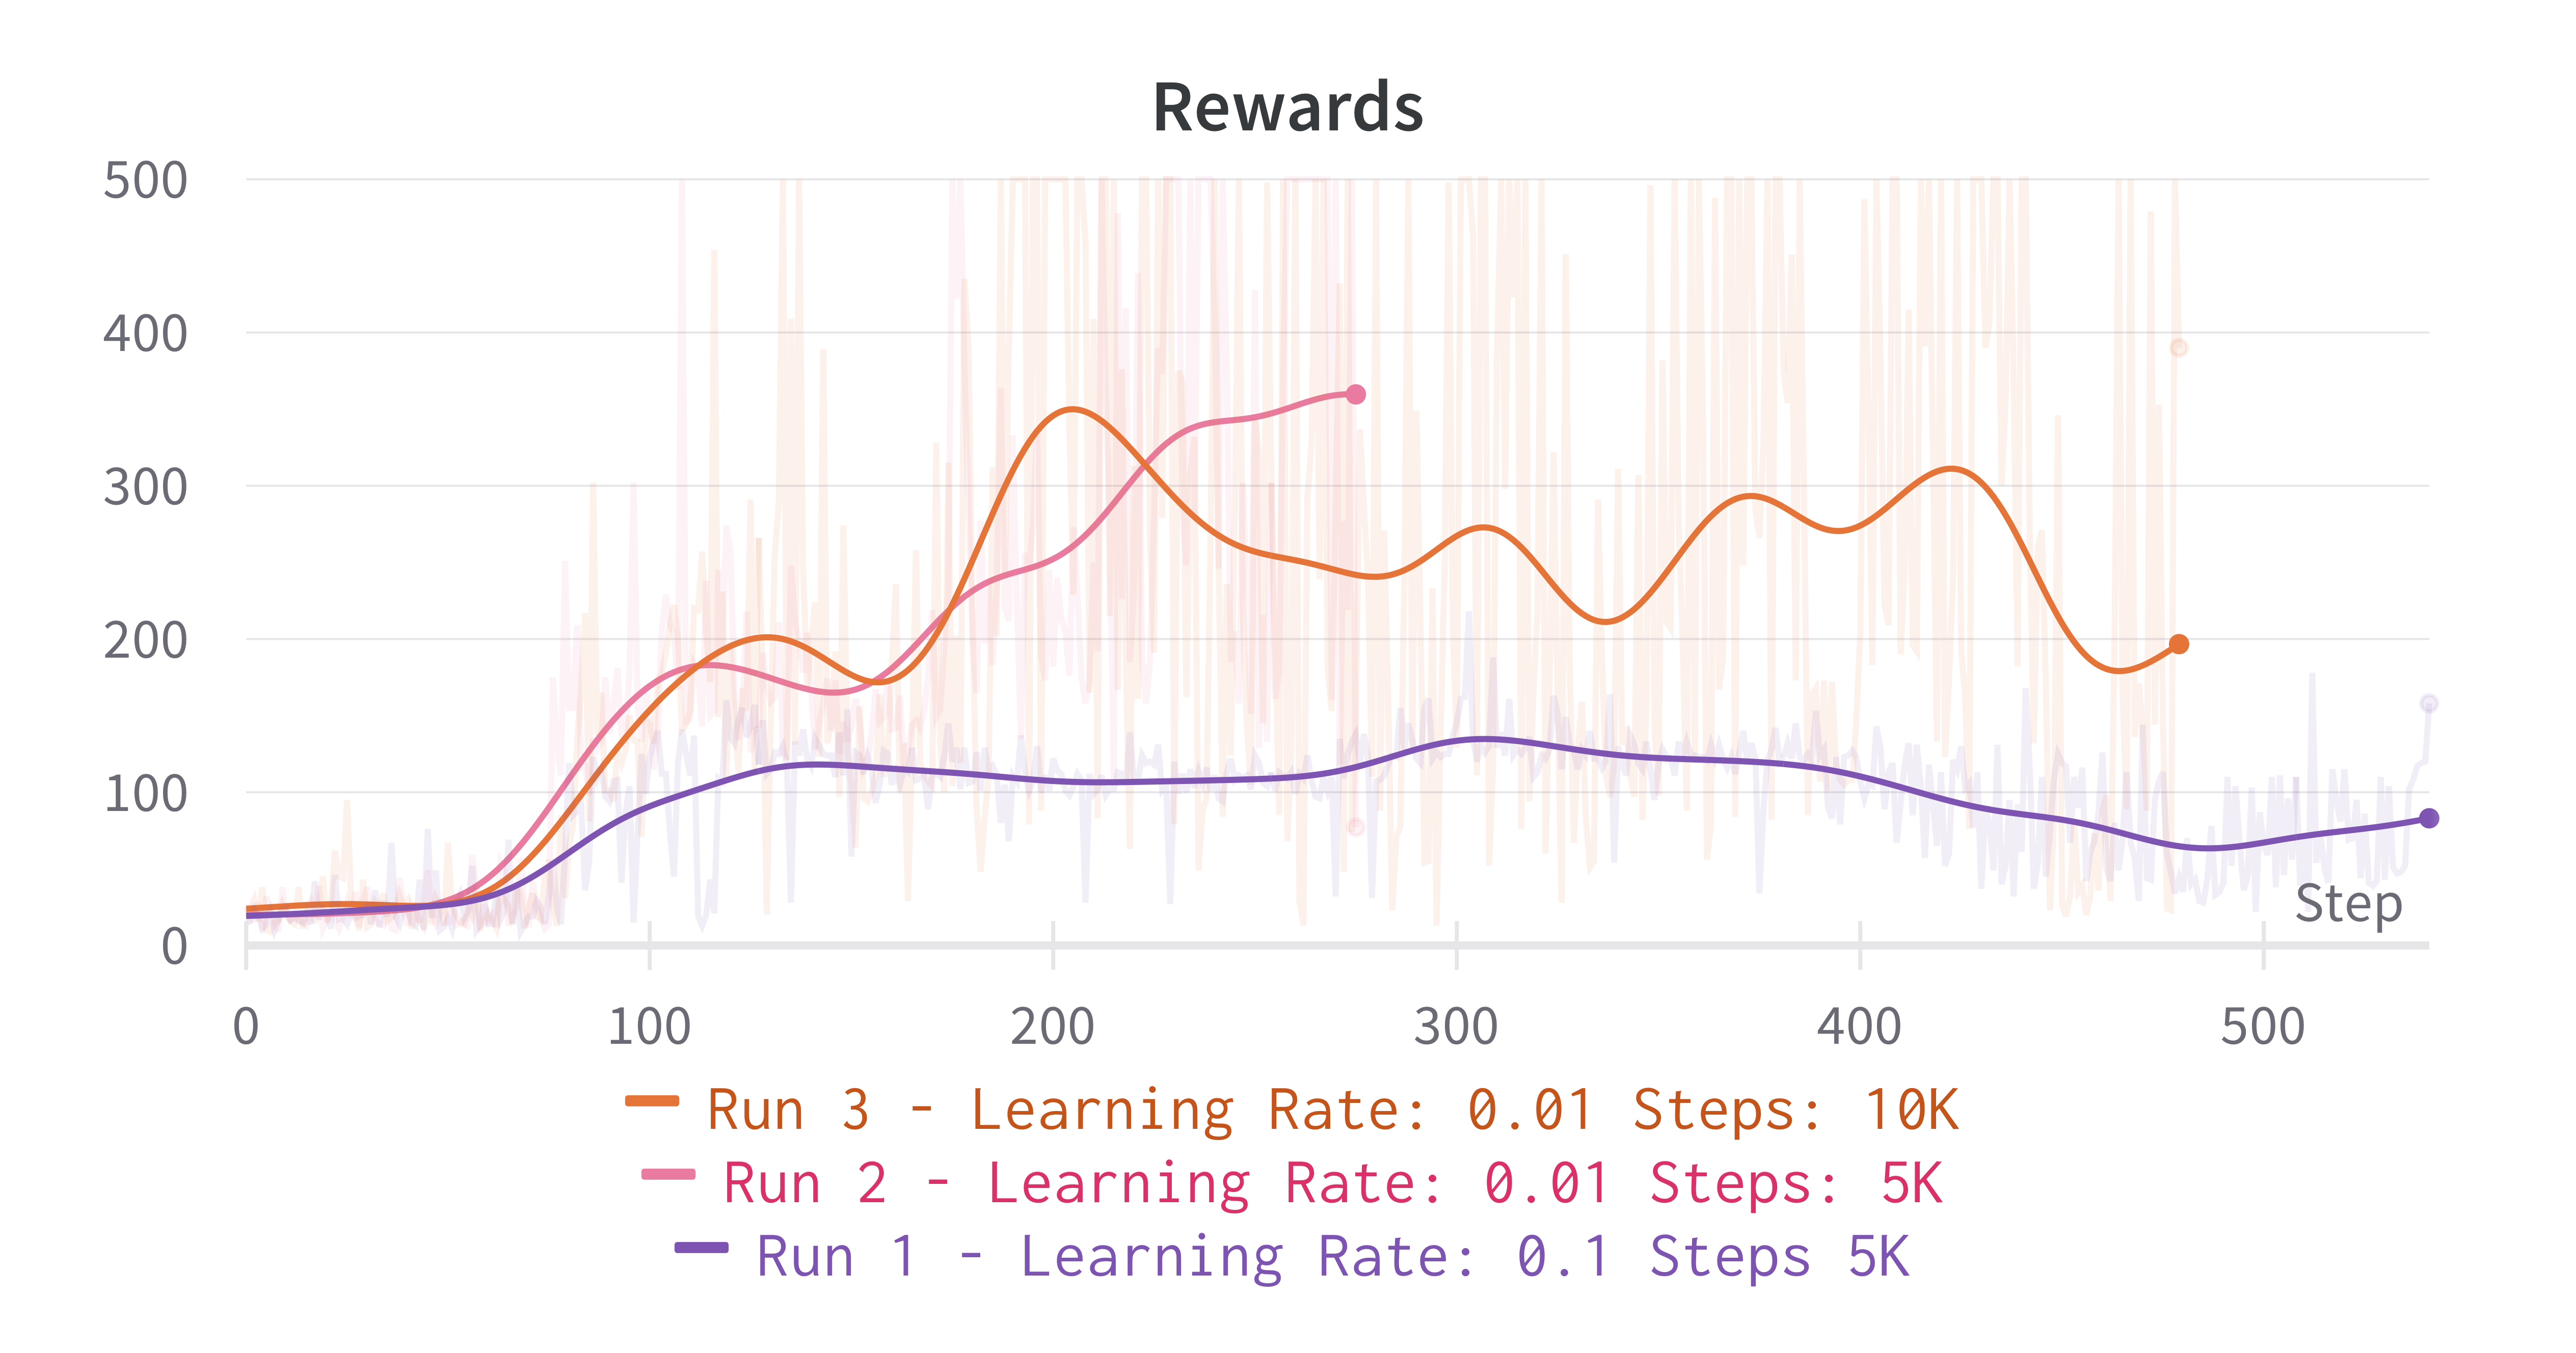
\includegraphics[width=1\textwidth]{charts/rewards_cartpole.png}
    \caption{Reward output for the cartpole experiment - Boltzmann }
    \end{figure}

%   \begin{figure}[H]
%   \centering
%   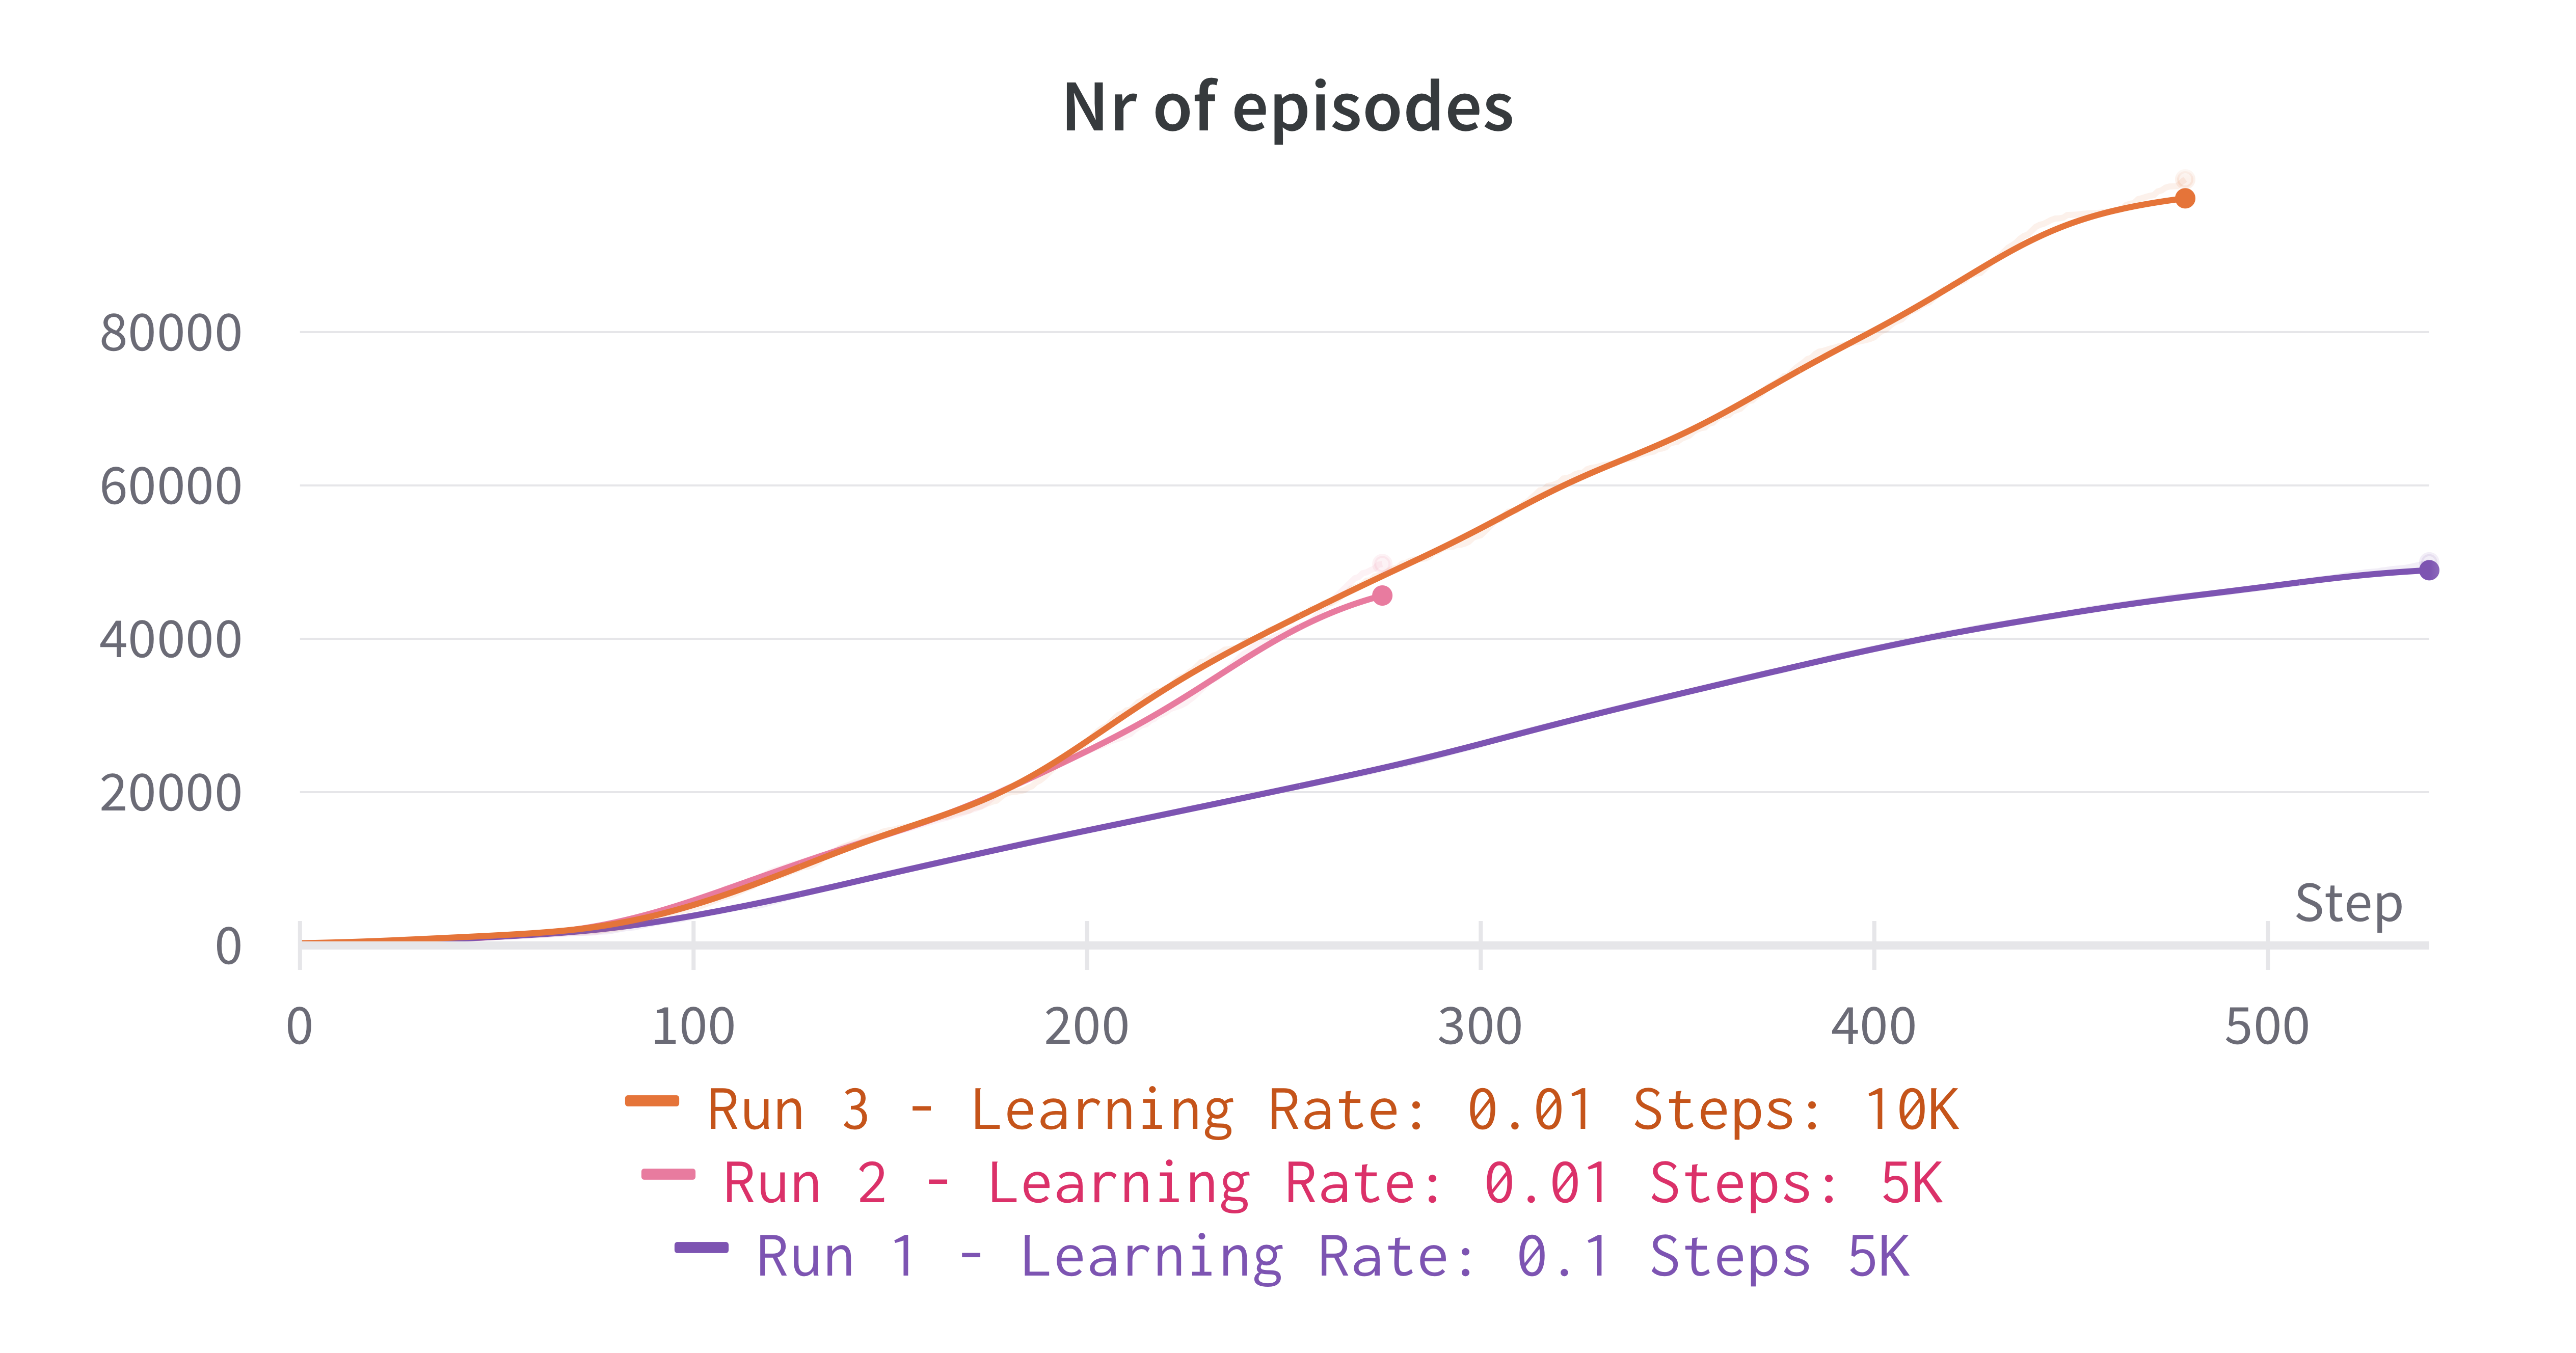
\includegraphics[width=1\textwidth]{charts/episodes_cartpole.png}
%   \caption{Number of episodes for the cartpole experiment}
%   \end{figure}
As can be seen from the above graphs, the learning rate of 0.01 shows much better results when compared to 0.1, although when the model was tested after 5000 steps the results were as follows:
\begin{table}[H]
    \begin{tabular}{ |p{2.2cm}|p{3cm}|p{3cm}| }
        \cline{2-3} 
        \multicolumn{1}{c}{} & \multicolumn{2}{|c|}{\Large \textbf{20 episodes test run}} \\
        \cline{2-3} 
        \multicolumn{1}{c}{} & \multicolumn{1}{|c|}{Learning Rate: 0.01} & \multicolumn{1}{|c|}{Learning Rate: 0.01}\\
        \multicolumn{1}{c}{} & \multicolumn{1}{|c|}{Steps 5000} & \multicolumn{1}{|c|}{Steps: 10000}\\
        \hline
        Episode 1 & 126.00  & 500.00\\
        Episode 2 & 121.00  & 500.00\\
        Episode 3 & 129.00  & 500.00\\
        Episode 4 & 124.00  & 500.00\\
        Episode 5 & 124.00  & 500.00\\
        Episode 6 & 123.00  & 500.00\\
        Episode 7 & 122.00  & 500.00\\
        Episode 8 & 123.00  & 500.00\\
        Episode 9 & 124.00  & 500.00\\
        Episode 10 & 123.00  &500.00 \\
        Episode 11 & 125.00  &500.00 \\
        Episode 12 & 116.00  &500.00 \\
        Episode 13 & 125.00  &500.00 \\
        Episode 14 & 126.00  &500.00 \\
        Episode 15 & 125.00  &500.00 \\
        Episode 16 & 127.00  &500.00 \\
        Episode 17 & 118.00  &500.00 \\
        Episode 18 & 125.00  &500.00 \\
        Episode 19 & 122.00  &500.00 \\
        Episode 20 & 119.00  &500.00 \\
        \hline
        \multicolumn{1}{c}{} & \multicolumn{1}{|c|}{\textbf{Average: 123.35}} & \multicolumn{1}{|c|}{\textbf{Average: 500.00}} \\
        \cline{2-3}
        \multicolumn{3}{c}{} 
    \end{tabular}
\end{table}
   
   As we can observe from the table, the training length can have a significant impact on the results, 
   in the case of the cartpole environment it helps to break harmfull correlations, stoping the cart from moving of the boundaries. 

   The second attempt uses a more common exploration policy, epsilon greedy, in this experiment the epsilon, learning rate and metric used were also varied.
   \begin{figure}[H]
       \centering
       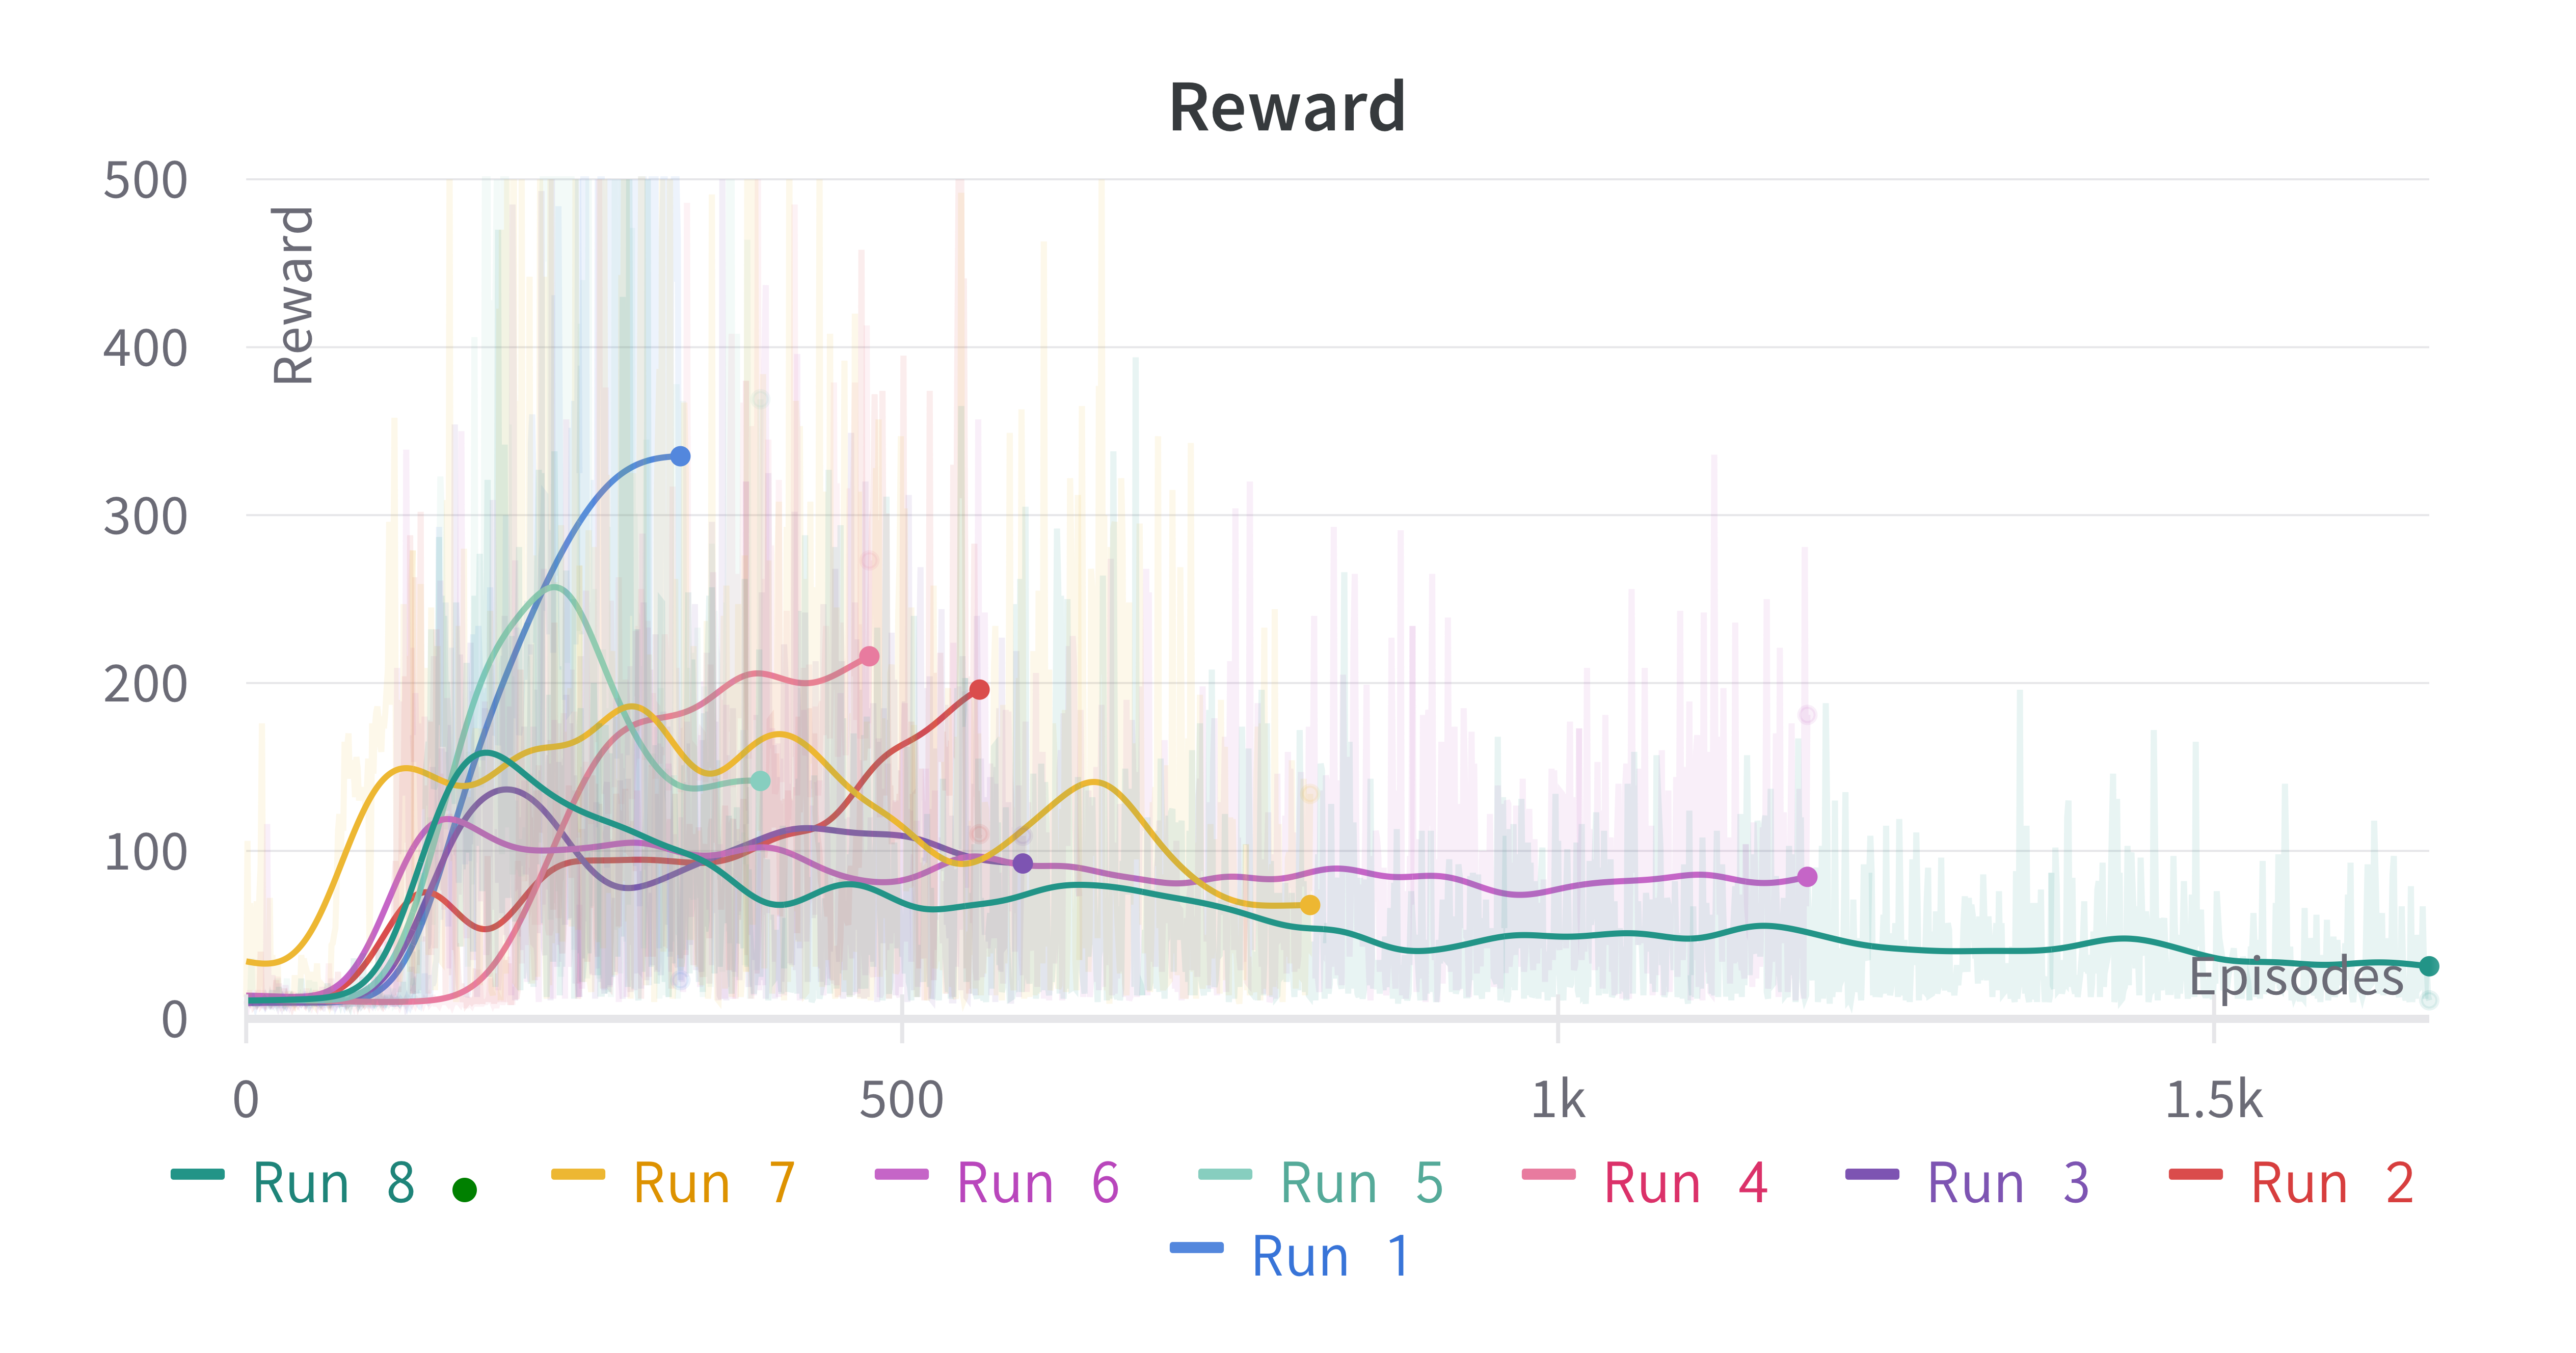
\includegraphics[width=1\textwidth]{charts/eps_greedy.png}
       \caption{Reward output for the cartpole experiment - epsilon greedy}
    \end{figure}
    
\begin{center}
    \begin{table}[H]
        \begin{tabular}{|l|l|l|l|l|l|l|l|l|}
        \hline
        Hyperparameters & Run 1 & Run 2 & Run 3 & Run 4 & Run 5    & Run 6  & Run 7 & Run 8    \\ \hline
        epsilon         & 0.1   & 0.1   & 0.1   & 0.1   & 0.1      & 0.1    & 0.2   & 0.3      \\ \hline
        learning rate   & 0.01  & 0.1   & 0.03  & 0.001 & 0.01     & 0.03   & 0.01  & 0.01     \\ \hline
        metric          & mae   & mae   & mae   & mae   & accuracy & mae    & mae   & mae      \\ \hline
        number of steps & 50000 & 50000 & 50000 & 50000 & 50000    & 100000 & 100000& 100000   \\ \hline
        \end{tabular}
    \end{table}
\end{center}
    
        \begin{table}[H]
        \begin{tabular}{l|l|l|l|l|l|l|l|l|}
        \cline{2-9}
                                         & Run 1 & Run 2 & Run 3 & Run 4 & Run 5    & Run 6& Run 7  & Run 8 \\ \hline
        \multicolumn{1}{|l|}{Episode 1}  & 500.00 & 31.00 & 47.00 & 390.00 & 500.00 & 88.00& 500.00 & 89.00\\
        \multicolumn{1}{|l|}{Episode 2}  & 500.00 & 28.00 & 49.00 & 338.00 & 500.00 & 87.00& 500.00 & 95.00\\
        \multicolumn{1}{|l|}{Episode 3}  & 500.00 & 85.00 & 33.00 & 500.00 & 500.00 & 84.00& 500.00 & 90.00\\
        \multicolumn{1}{|l|}{Episode 4}  & 500.00 & 85.00 & 26.00 & 166.00 & 500.00 & 90.00& 500.00 & 92.00\\
        \multicolumn{1}{|l|}{Episode 5}  & 500.00 & 28.00 & 51.00 & 210.00 & 500.00 & 91.00& 500.00 & 88.00\\
        \multicolumn{1}{|l|}{Episode 6}  & 500.00 & 28.00 & 57.00 & 307.00 & 500.00 & 88.00& 500.00 & 93.00\\
        \multicolumn{1}{|l|}{Episode 7}  & 500.00 & 34.00 & 41.00 & 335.00 & 500.00 & 86.00& 500.00 & 95.00\\
        \multicolumn{1}{|l|}{Episode 8}  & 500.00 & 27.00 & 22.00 & 343.00 & 500.00 & 91.00& 500.00 & 92.00\\
        \multicolumn{1}{|l|}{Episode 9}  & 500.00 & 85.00 & 80.00 & 307.00 & 500.00 & 86.00& 500.00 & 87.00\\
        \multicolumn{1}{|l|}{Episode 10} & 500.00 & 33.00 & 21.00 & 500.00 & 500.00 & 92.00& 500.00 & 92.00\\
        \multicolumn{1}{|l|}{Episode 11} & 500.00 & 28.00 & 26.00 & 139.00 & 500.00 & 29.00& 500.00 & 90.00\\
        \multicolumn{1}{|l|}{Episode 12} & 500.00 & 83.00 & 90.00 & 437.00 & 500.00 & 87.00& 500.00 & 87.00\\
        \multicolumn{1}{|l|}{Episode 13} & 500.00 & 30.00 & 75.00 & 341.00 & 500.00 & 90.00& 500.00 & 91.00\\
        \multicolumn{1}{|l|}{Episode 14} & 500.00 & 33.00 & 56.00 & 500.00 & 500.00 & 88.00& 500.00 & 90.00\\
        \multicolumn{1}{|l|}{Episode 15} & 500.00 & 88.00 & 41.00 & 493.00 & 500.00 & 87.00& 500.00 & 93.00\\
        \multicolumn{1}{|l|}{Episode 16} & 500.00 & 31.00 & 88.00 & 500.00 & 500.00 & 86.00& 500.00 & 91.00\\
        \multicolumn{1}{|l|}{Episode 17} & 500.00 & 29.00 & 39.00 & 500.00 & 500.00 & 81.00& 500.00 & 93.00\\
        \multicolumn{1}{|l|}{Episode 18} & 500.00 & 35.00 & 33.00 & 500.00 & 500.00 & 87.00& 500.00 & 89.00\\
        \multicolumn{1}{|l|}{Episode 19} & 500.00 & 83.00 & 67.00 & 340.00 & 500.00 & 94.00& 500.00 & 93.00\\
        \multicolumn{1}{|l|}{Episode 20} & 500.00 & 32.00 & 77.00 & 242.00 & 500.00 & 87.00& 500.00 & 92.00\\ \hline
        \multicolumn{1}{|l|}{\textbf{Average}} & 500.00 & 46.80 & 50.95 & 369.40 & 500.00 & 84.95 & 500.00 &91.10 \\
        \hline
    \end{tabular}
    \caption{test} % TODO: #1 label
    \end{table}

    When comparing the two approaches, it is clear that the more common epsilon greedy approach was more successfull in solving the cartpole environment, achieving the maximum of 500 points in 50000 steps.

    As can be observed by the table containing the average reward for 20 test episodes, we can observe that both run 1 and run 5 were successfull with 50000 steps, followed by run 4 with close scores.
    Both run 1 and 5 have 0.01 as the learning rate and only vary the metric used, any learning rate above 0.01 tested yelded low scores, when testing varying epsilons it was possible to solve the environment with double the steps, 
    the results also demonstrate that setting random exploration to values higher than 20\% couldn't be solved under the 10000 steps.

    The conclusion drawn show that the most suitable parameters are:
    \begin{itemize}
        \item \textbf{epsilon} = 0.1
        \item \textbf{learning rate} = 0.01
        \item \textbf{metric} = mae
        \item \textbf{number of steps} = 50000
    \end{itemize}
        
   \section{2D Environment Outcomes}
%%%%%%% MIGHT NOT BELONG HERE %%%%%%%%%%
When first implementing the 2D environemnt using the keras-rl library, it was found that the library doesn't support the use of Multidiscrete action spaces, 
an attempt to implement this environment using tensorflow Agents yelded the same results:


$\makebox[\linewidth]{"ValueError: Only scalar actions are supported now"}$

Given this, it was necessary to implement a custom learning implementation using the Keras API.
%%%%%%% MIGHT NOT BELONG HERE %%%%%%%%%%

The 2D environment was a big challenge to develop, this is due to the big jump in complexity in comparison with a simple, well known and documented environment such as the cartpole.
The 2D environment required a custom 2D environment and the implementation of this with the physics engine. When this obstacle was overcome, the second major challenge was to implement the learning algorithm
and be able to control the 8 joints simultaniously.

Once the learning algorithm was fully implemented, the reward system and hyperparameters needed to be tested and tuned, this shows the complexity of reinforcement learning. While many itterations over the reward system and hyperparameters were made, given the limited time and resources a full walking motion could not have been achieved.
Although, the results obtained with experientation were helpfull in understading the impact of the changes in the reward system.
\subsection*{Results}
\begin{figure}[H]
    \centering
    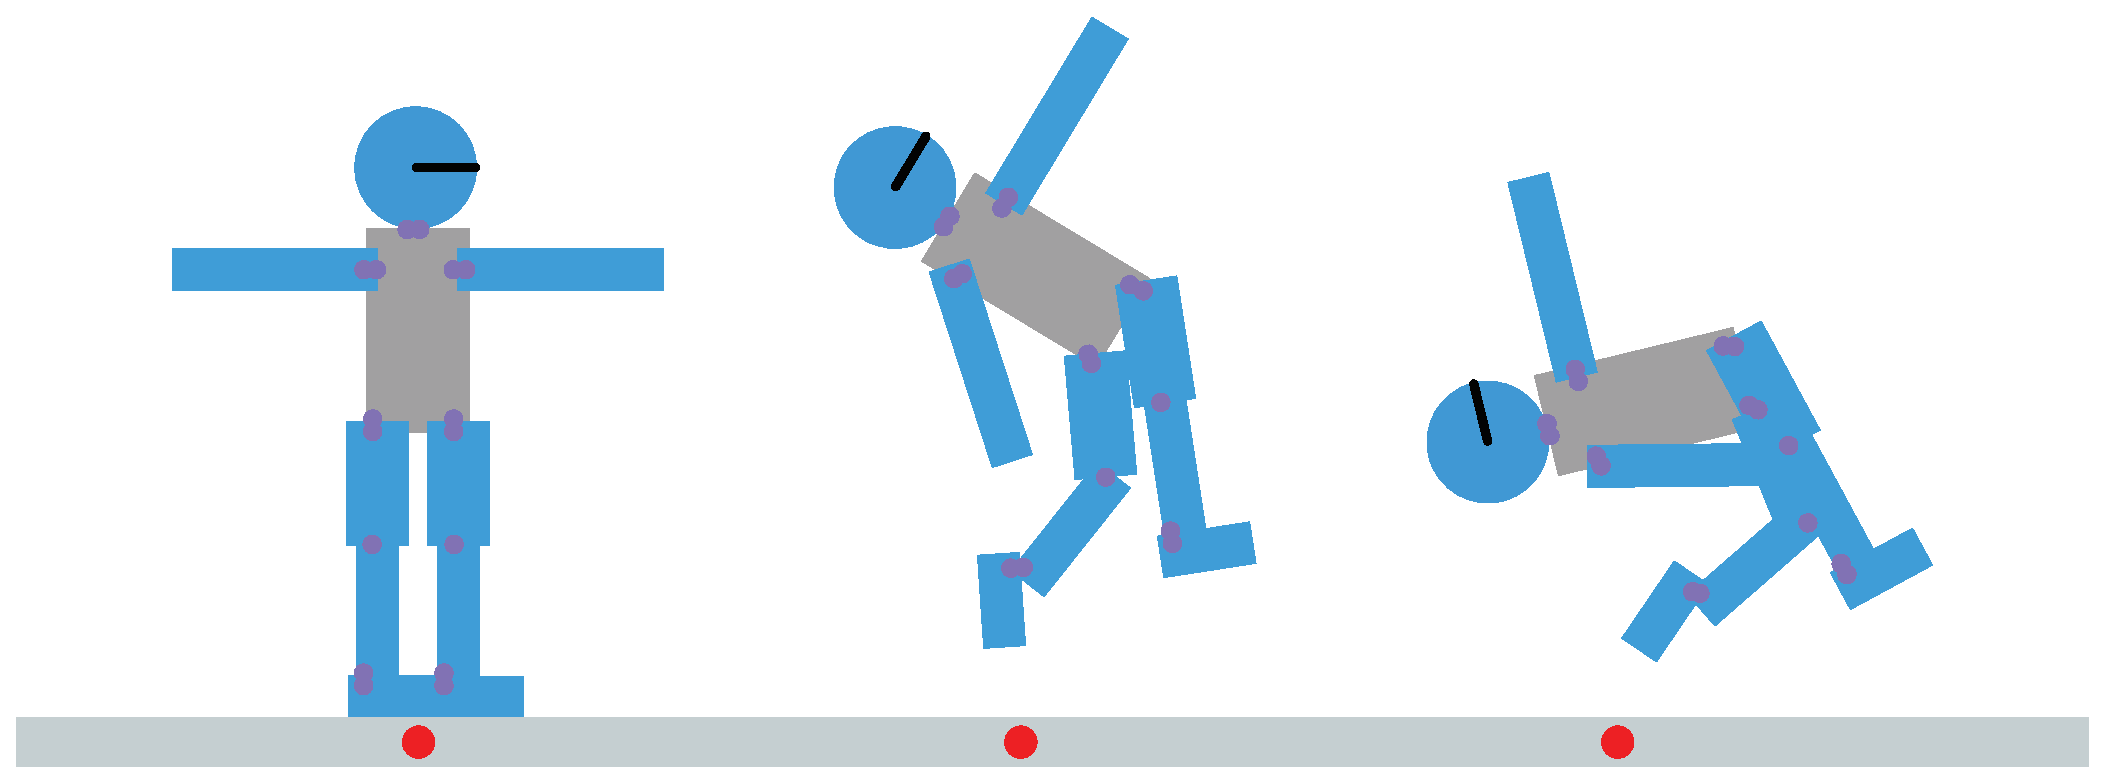
\includegraphics[scale=0.3]{2d_walk_199_episodes}
    \caption{Simulation of 2D environment after 199 episodes}
\end{figure}
\begin{figure}[H]
    \centering
    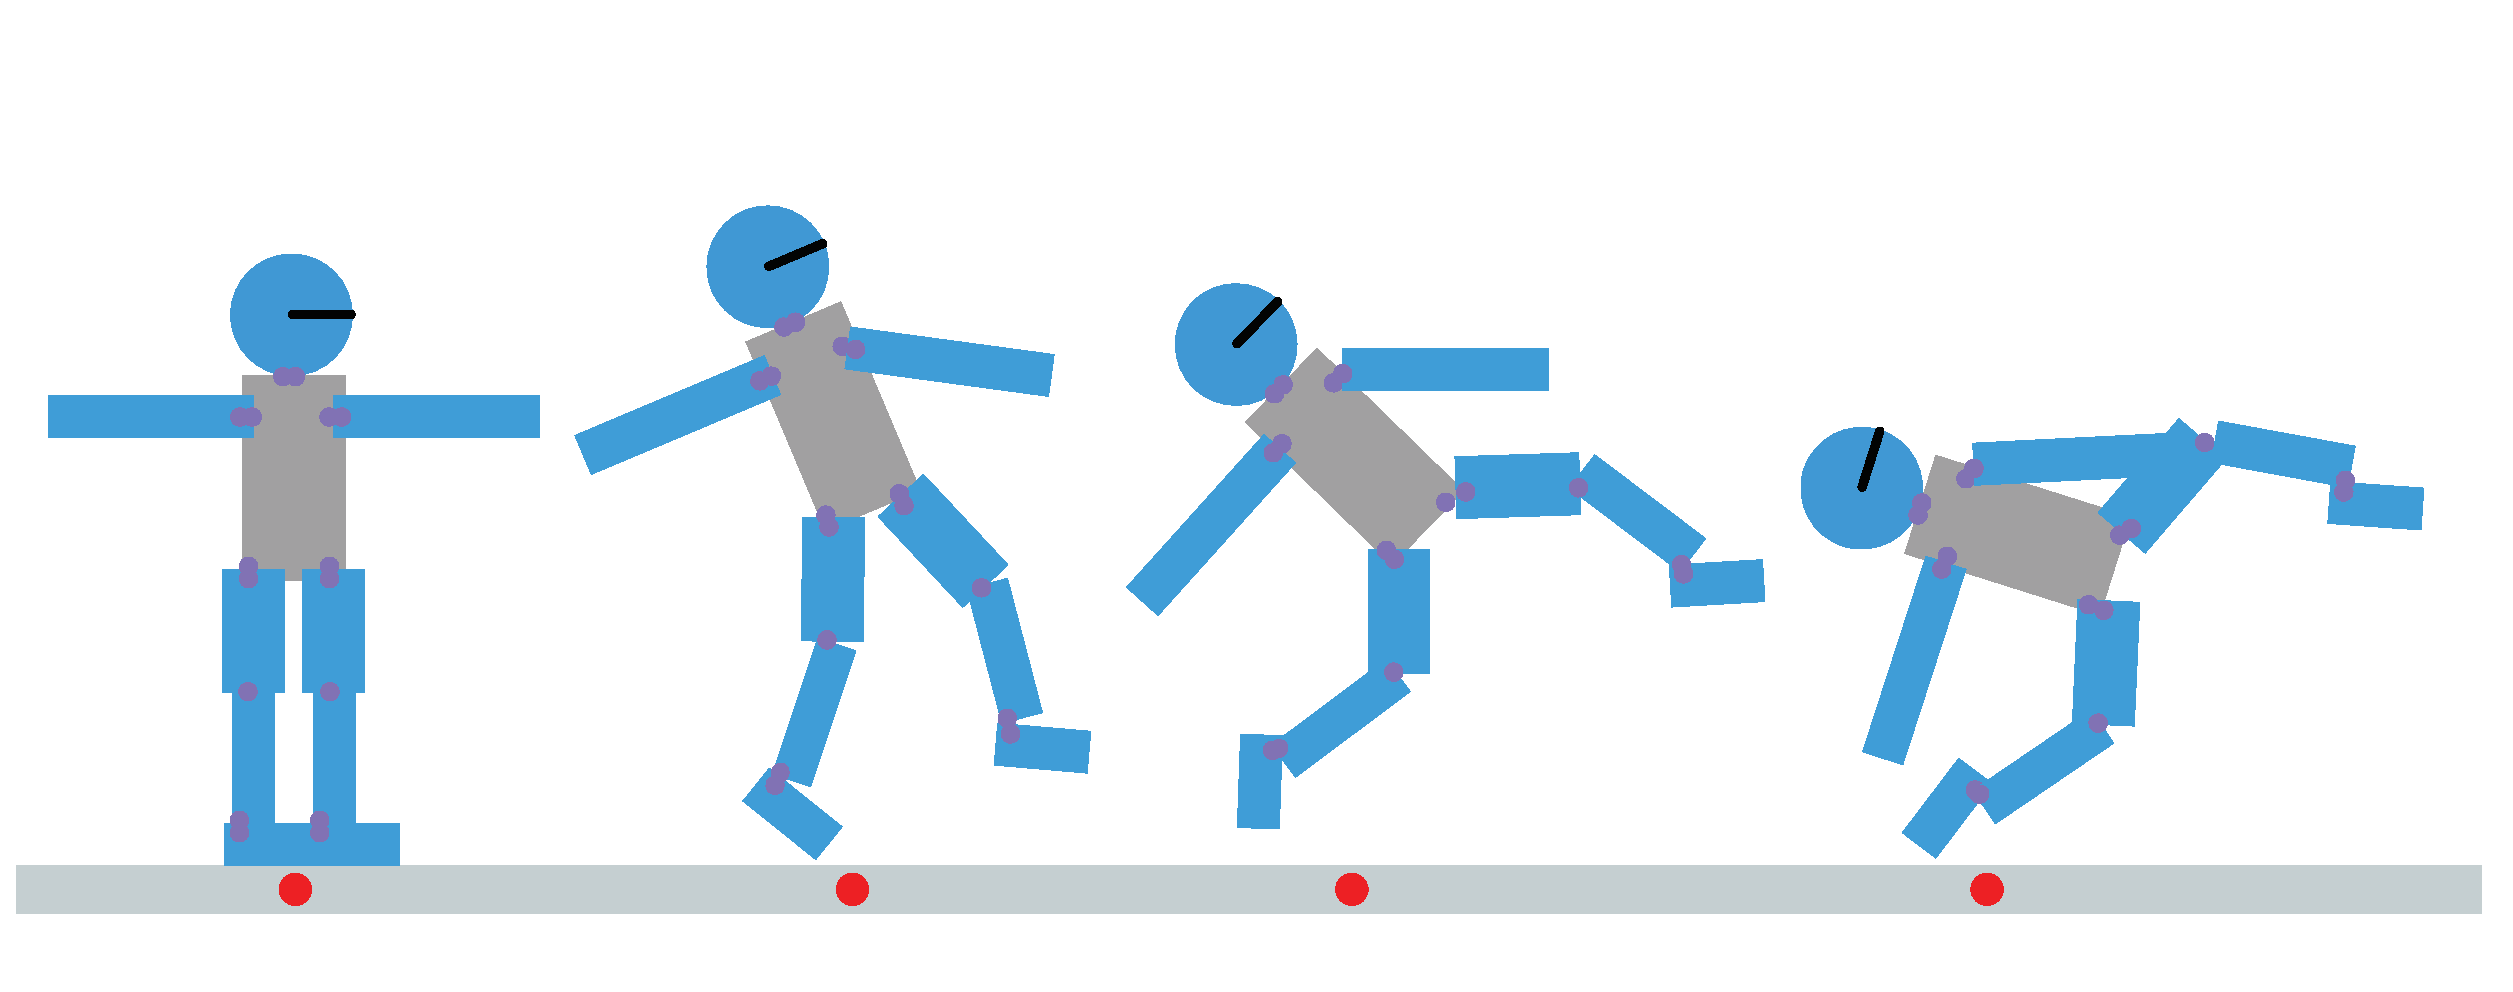
\includegraphics[scale=0.3]{2d_walk_10651_episodes}
    \caption{Simulation of 2D environment after 10651 episodes}
\end{figure}

\begin{table}[H]
    \centering
    \begin{tabular}{|ll|}
    \hline
    \multicolumn{2}{|c|}{Hyperparameters}                              \\ \hline
    \multicolumn{1}{|l|}{gamma}                  & 0.99                \\ \hline
    \multicolumn{1}{|l|}{learning rate}          & 0.01                \\ \hline
    \multicolumn{1}{|l|}{epsilon maximum}        & 0.1                 \\ \hline
    \multicolumn{1}{|l|}{epsilon minimum}        & 0.01                \\ \hline
    \multicolumn{1}{|l|}{batch size}             & 64                  \\ \hline
    \multicolumn{1}{|l|}{units per hidden layer} & 128                 \\ \hline
    \multicolumn{1}{|l|}{loss function}          & mean absolute error \\ \hline
    \end{tabular}
\end{table}
After 10000 episodes we start to observe how the agent starts to learn to move forward as it yelds the most rewards as opposed to the example of 199 episodes where the agent would jump and fall almost in the starting position.
From performing a parameter importance analysis on a larger number of runs using the wandb logger, the perceived notions are confirmed as can be seen bellow:
\begin{figure}[H]
    \centering
    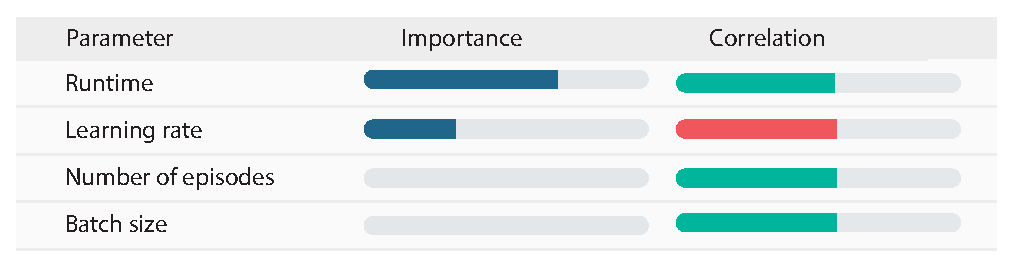
\includegraphics[scale=0.8]{parameter_importance_2D}
    \caption{Parameter importance analysis of the 2D environment}
\end{figure}
%this graph is shit

\section{3D Environment Outcomes}

\section{Reward Function}

